\documentclass[12pt]{article}

\usepackage{listings}
\usepackage{pdfpages}
\usepackage[english]{babel}
\usepackage[utf8x]{inputenc}
\usepackage[T1]{fontenc}
\usepackage{rotating}
\usepackage{float}
\usepackage{tikz}
\usepackage[a4paper,top=3cm,bottom=2cm,left=3cm,right=3cm,marginparwidth=1.75cm]{geometry}

\usepackage{amsmath}
\usepackage{graphicx}
\usepackage[colorinlistoftodos]{todonotes}
\usepackage{hyperref}
\hypersetup{
    colorlinks = true,
    citecolor=black,
    linktoc=all,
    filecolor=black,
    linkcolor=black,
    urlcolor=black
}

\usepackage{listings}
\usepackage{color}

\definecolor{mygreen}{rgb}{0,0.6,0}
\definecolor{mygray}{rgb}{0.5,0.5,0.5}
\definecolor{mymauve}{rgb}{0.58,0,0.82}

\lstset{ %
  backgroundcolor=\color{white},   % choose the background color; you must add \usepackage{color} or \usepackage{xcolor}; should come as last argument
  basicstyle=\footnotesize,        % the size of the fonts that are used for the code
  breakatwhitespace=false,         % sets if automatic breaks should only happen at whitespace
  breaklines=true,                 % sets automatic line breaking
  captionpos=b,                    % sets the caption-position to bottom
  commentstyle=\color{mygreen},    % comment style
  deletekeywords={...},            % if you want to delete keywords from the given language
  escapeinside={\%*}{*)},          % if you want to add LaTeX within your code
  extendedchars=true,              % lets you use non-ASCII characters; for 8-bits encodings only, does not work with UTF-8
  frame=single,	                   % adds a frame around the code
  keepspaces=true,                 % keeps spaces in text, useful for keeping indentation of code (possibly needs columns=flexible)
  keywordstyle=\color{blue},       % keyword style
  language=SQL,                 % the language of the code
  morekeywords={*,...},           % if you want to add more keywords to the set
  numbers=left,                    % where to put the line-numbers; possible values are (none, left, right)
  numbersep=5pt,                   % how far the line-numbers are from the code
  numberstyle=\tiny\color{mygray}, % the style that is used for the line-numbers
  rulecolor=\color{black},         % if not set, the frame-color may be changed on line-breaks within not-black text (e.g. comments (green here))
  showspaces=false,                % show spaces everywhere adding particular underscores; it overrides 'showstringspaces'
  showstringspaces=false,          % underline spaces within strings only
  showtabs=false,                  % show tabs within strings adding particular underscores
  stepnumber=1,                    % the step between two line-numbers. If it's 1, each line will be numbered
  stringstyle=\color{mymauve},     % string literal style
  tabsize=2,	                   % sets default tabsize to 2 spaces
  title=\lstname                   % show the filename of files included with \lstinputlisting; also try caption instead of title
}

\title{Database Design Term Project}
\author{Ciaran Roche, Mathana Nair Sreedaran}

\begin{document}

\begin{titlepage}
    \centering
    \includegraphics[width=0.15\textwidth]{wit-logo.JPG}\par\vspace{1cm}
    {\scshape\LARGE Waterford Institute of Technology \par}
    \vspace{1cm}
    {\scshape\Large Database Design Term Project\par}
    \vspace{1.5cm}
    {\huge\bfseries Movie Sequel DB\par}
    \vspace{2cm}
    {\Large\itshape Ciaran Roche(20037160)\par}
    {\Large\itshape Mathana Nair Sreedaran (20069456)\par}
    \vfill
% Bottom of the page
    {\large \today\par}
\end{titlepage}
\newpage
\pagenumbering{gobble}
\tableofcontents

\newpage
\pagenumbering{arabic}

\begin{abstract}
    The purpose of this paper is to design and develop a database using MySQL Workbench. The following is practical work as part of the Database Design module in BSc.(Hons) Applied Computing, at Waterford Institute of Technology. A unique project topic was selected. A proposal was submitted, a demonstration of the project was performed and project design documents and database scripts were presented.
\end{abstract}

\section{Introduction}
The chosen area or topic for this project is movies. The aim of the project was to create a movie database containing data essential to all users ranging from the average user looking for the description of a movie to somebody from the entertainment industry who is looking for additional information related to a movie such as the band or artiste of a song from the movie. The information included in the database covers a wide range of elements that can be of use to anybody seeking information related to a movie. 
    
\section{Project Description}
Movies are a form of entertainment to many people. Making a movie requires the collaborative effort of people with varied expertise. For example, producers are needed to plan and coordinate various aspects of a movie and the actors and actresses give life to the movie under direction of the director.

Simply put, a movie and the movie industry contain much data which should be made available to anybody who seeks it. This is facilitated with the use of a database. By centralising data in an orderly manner, users may access it efficiently.

The major functions of this database include the retrieval of information relevant to a movie such as the movie description, rating and runtime and other information which are attributed to a movie such as the soundtrack, songs of the soundtrack and artiste or band who played those songs. The people behind the movie are also included along with their respective roles such as actor, director and writer. All the tables in the database can be found in the Table Design section of this report. 

\newpage
\section{Model}
The model was designed using Visual Paradigm and underwent multiple iterations. The model is shown on the following page;
\begin{sidewaysfigure}
    \centering
    \includegraphics{Class_Diagram1.png}
\end{sidewaysfigure}

\newpage
\section{Table Design}
The following are tables which resulted from the preceding model with details such as primary keys, foreign keys and integrity constraints.
\includepdf[pages={1,2}]{sql-tables.pdf}

\section{SQL Scripts}
\subsection{Create Database Script}

The complete copy of all scripts can be found at the following link:\newline \href{https://github.com/ciaranRoche/mySQL-movie-db}{https://github.com/ciaranRoche/mySQL-movie-db} \newline

Below is an example of a create table script. The complete script can be found at this \href{https://github.com/ciaranRoche/mySQL-movie-db/blob/master/database-createtable-script.sql}{link.}

\begin{lstlisting}[language=SQL]
drop database sequelmovie;
create database sequelmovie;
use sequelmovie;

create table movie(
    movieID int(5) not null,
    movieTitle varchar(50) not null,
    movieDesc varchar(150),
    movieReleaseDate date,
    movieRuntime int(3) check (movieRuntime > 25),
    movieCertificate varchar(4) check (movieCertificate in
    ('N/A','PG','12','12A','15','15A','16','18')),
    movieRating int(1) check (movieRating > 0 and movieRating <= 5),
    constraint movie_pk primary key (movieID)
)engine innodb;

\end{lstlisting}

\subsection{Triggers Script}
Below are the scripts for triggers;\newline\newline
The trigger below ensures the movie runtime is above 25. 
\begin{lstlisting}[language=SQL]
delimiter $$
create trigger before_movie_insert_movieRuntime before insert on movie
for each row
begin
	if new.movieRuntime <= 25 then
	signal sqlstate '42000'
	set message_text = 'Check constraint on movieRuntime in table movie failed. Runtime too short';
	end if;
end$$
delimiter ;
\end{lstlisting}

\newpage
The trigger below ensures the movie certificate adheres to those defined by the Irish Film Classification Office.
\begin{lstlisting}[language=SQL]
delimiter $$
create trigger before_movie_insert_movieCertificate before insert on movie
for each row
begin
	if new.movieCertificate not in ('N/A','PG','12','12A','15','15A','16','18') then
    signal sqlstate '41000'
    set message_text = 'Check constraint on movieCertificate in table movie failed. Only Irish ratings';
    end if;
end$$
delimiter ;
\end{lstlisting}

The following trigger ensures movie ratings are between 1 to 5 only.
\begin{lstlisting}[language=SQL]
delimiter $$
create trigger before_movie_insert_movieRating before insert on movie
for each row
begin
	if (new.movieRating < 1) OR (new.movieRating > 5) then
	signal sqlstate '42000'
	set message_text = 'Check constraint on movieRating in table movie failed. Outrageous rating my good sir/madame';
	end if;
end$$
delimiter ;

\end{lstlisting}

\newpage
\subsection{Insert Script}
Below is an example of a movie insert script. The complete scripts can be found at this \href{https://github.com/ciaranRoche/mySQL-movie-db/blob/master/database-insert-script.sql}{link.}
\begin{lstlisting}[language=SQL]
use sequelmovie;

insert into movie values (0001, 'The Shawshank Redemption',
'Two imprisoned men bond over a number of years', 
'1994-10-14', 142, '18', '4.5');

\end{lstlisting}

\subsection{Queries Script}
Below is an example of a few query scripts. The complete scripts can be found at this \href{https://github.com/ciaranRoche/mySQL-movie-db/blob/master/database-queries-scripts.sql}{link.}
\begin{lstlisting}[language=SQL]
use sequelmovie;

describe movie;

select movieTitle as Title, movieDesc 
as Description, movieReleaseDate as 'Release Date', movieRuntime as Runtime
from movie;

update person
	set personPicture = ifnull(personPicture, 'http://www.uidownload.com/files/478/82/442/error-404-page-not-found-icon.jpg');

delete from movie
where movieTitle = 'Alien';

alter table movie
change movieDesc moviePlot varchar(150);
\end{lstlisting}

\newpage
\subsection{Views Script}
Views were created with different users in mind. The name of the views indicate which tables it uses. Below are the scripts to create views; 
\begin{lstlisting}[language=SQL]
use sequelmovie;

create view movie_v_trailer as
  select movieTitle, trailerURL
  from movie, trailer
  where movieID = t_movieID;

create view movie_v_trailer_poster as
  select movieTitle, trailerURL, posterLink
  from movie, trailer, poster
  where movieID = t_movieID and movieID = p_movieID;

create view movie_v_soundtrack as
  select movieTitle, soundtrackName
  from movie, soundtrack
  where movieID = m_movieID;

create view movie_v_genre as
  select movieTitle, genreType
  from movie, genre, movie_genre
  where movieID = m_movieID and g_genreID = genreID;

create view soundtrack_v_song as
  select soundtrackName, songName
  from soundtrack, song, soundtrack_song
  where soundtrackID = soundtrack_soundtrackID and song_songID=songID;

create view movie_v_actors as
  select movieTitle, personFirstName, personLastName, roleDesc
  from movie, person, role
  where movieID = m_movieID and p_personID = personID;

create view movie_v_studio as
  select movieTitle, studioName
  from movie, studio, movie_studio
  where movieID = m_movieID and s_studioID = studioID;
\end{lstlisting}


\newpage
\section{ER Diagram}
The ER diagram generated by reverse engineering the database and is shown in the following page;

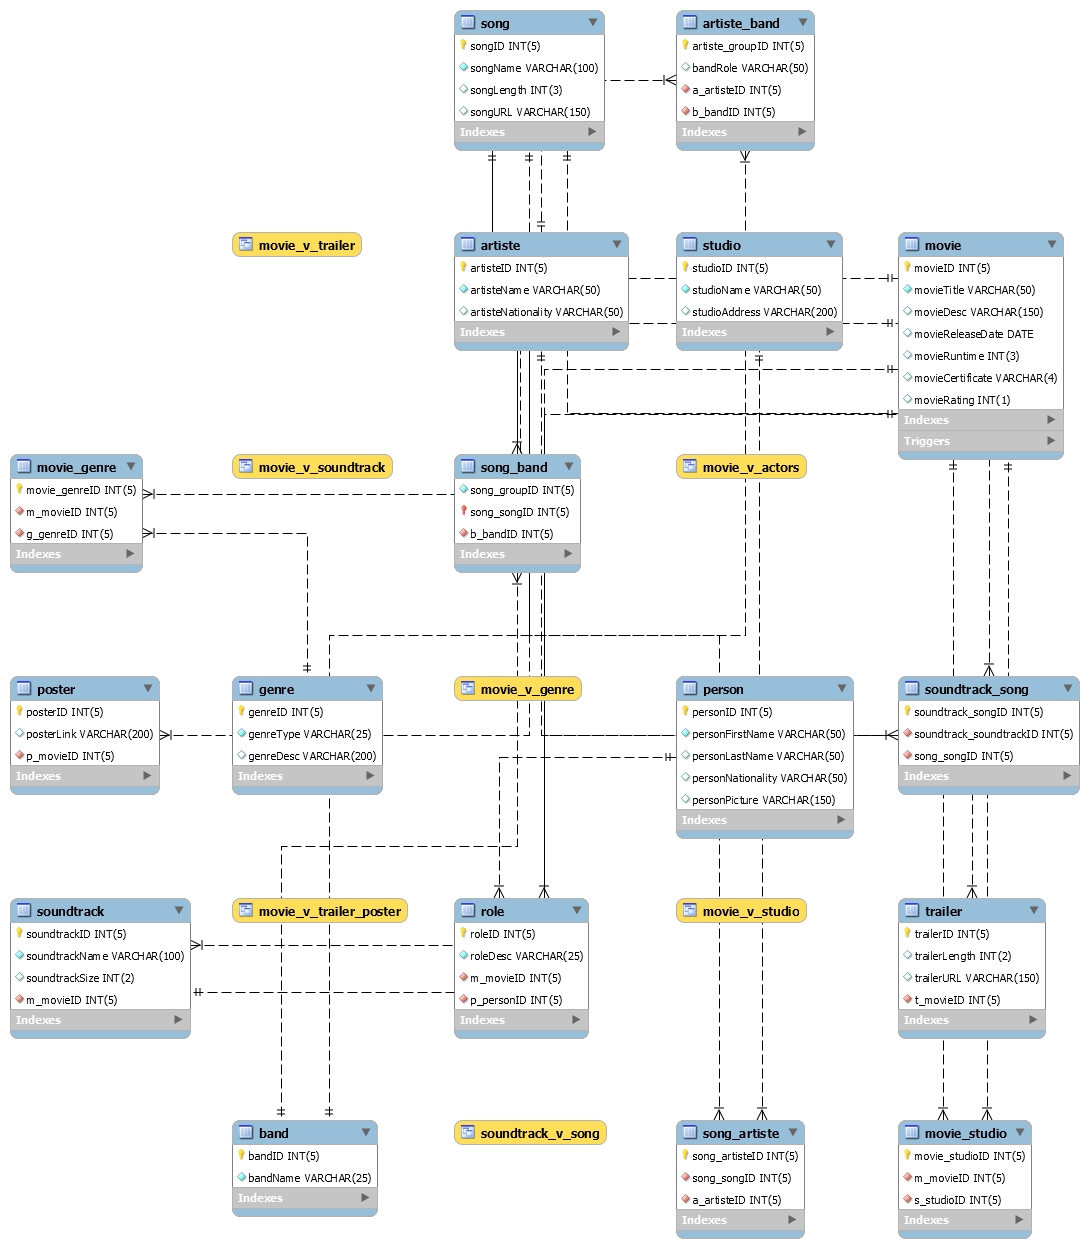
\includepdf[pages={1}]{er-diagram.pdf}

\newpage
\section{Conclusion}
In conclusion, the aim of the project to build a movie database was achieved. Much research was done to obtain movie data to populate the database. An open API (Application Program Interface) from The Open Movie Database, which returned data from IMDb, was used. Information not supplied by the API was sourced manually. A Python script was written to automate the population of the database. However, due to time constraints, the script was not used. It can be found at this \href{https://github.com/ciaranRoche/mySQL-movie-db/tree/master/snake}{link.}\newline\newline
All scripts were tested thoroughly to ensure they produced the intended output. Overall, a greater understanding of SQL with the use of MySQL workbench was obtained. In addition, the process of researching and building a database was learnt. 

\end{document}

